%!TEX root = ../thesis.tex
%*******************************************************************************
%****************************** Second Chapter *********************************
%*******************************************************************************

\chapter{Simple 1-Dimensional Problem}

\ifpdf
    \graphicspath{{Chapter2/Figs/Raster/}{Chapter2/Figs/PDF/}{Chapter2/Figs/}}
\else
    \graphicspath{{Chapter2/Figs/Vector/}{Chapter2/Figs/}}
\fi


\section{Outlining of Basic Principles}

% Uncomment this line, when you have siunitx package loaded.
By constraining $\bm{x}$ to one dimension allows for the problem to be simplified. Suppose ${f(x)=\sin(x)+0.05x^2}$ with ${x\in [-10, 10]}$ as shown in Figure~\ref{fig:firstFunction}. In this range, there are multiple minima with only one global minimum. The task here is to successfully locate the minima situated at -1.428. Three methods will be used here: $\text{fminbound}$ \cite{2020SciPy-NMeth}, greatest uncertainty active learning, and problem specific active learning (explained in Section~\ref{sssec:Active Learning}). $\epsilon$ will be chosen to be independent of $x$ and $y$ and fit a normal distribution such that ${\epsilon\sim N(0, 0.2^2)}$.

\begin{figure}[htbp!] 
\centering    
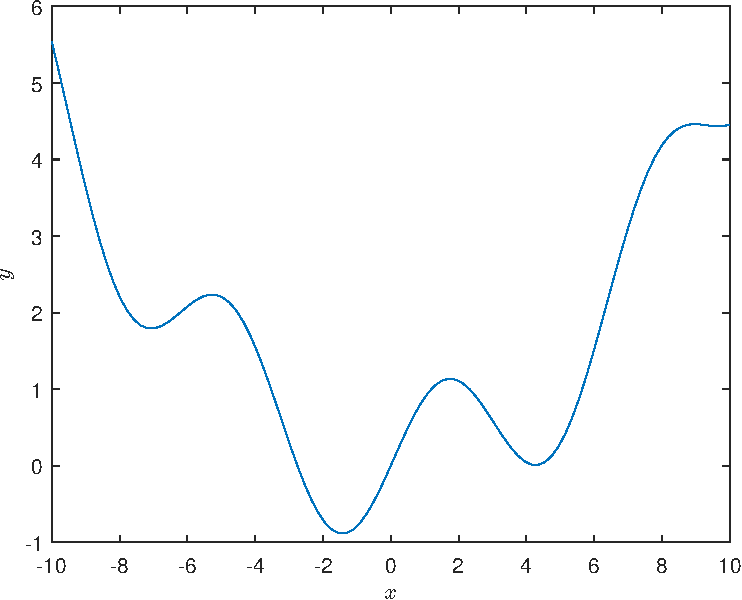
\includegraphics[width=1.0\textwidth]{firstFunction.pdf}
\caption[First Function]{$y = \sin(x) + 0.005x^2$ with $x\in [-10, 10]$}
\label{fig:firstFunction}
\end{figure}

\subsection{Algorithms}
\label{ssec: algorithms}
\subsubsection{fminbound}
fminbound is a function included in the scipy optimisation library \cite{2020SciPy-NMeth}. It uses Brent's method allowing it to be quick in situations where labelling is quick and error is low.

\subsubsection{Greatest Uncertainty Active Learning}
Without a basis for implementing a probability model on curve fitting, regions with maximum scarcity of samples will be chosen. In practice, this means for $n+1$ samples within the range $[\alpha, \beta]$, the sample $s_i$, $i\in\mathbb{Z}$, $i\in[0, n]$ will fall according to (\ref{eq: UAL}). A smoothing spline fit will be used for interpolation identically to problem specific active learning in Section~\ref{sssec:Active Learning}.

\begin{equation}
  \label{eq: UAL}
  s_i=\alpha+i\frac{\beta-\alpha}{n}
\end{equation}

\subsubsection{Problem Specific Active Learning}
\label{sssec:Active Learning}
This methodology has two underlying core principles: sparse areas reveal the most information and minimal areas reveal information to the location of minima. Combining these allows for better decision making in selecting the next sample. A smoothing spline is used to interpolate providing $e(x)$ in (\ref{eq: height}). Functions $h(x)$ and $p(x)$ (see (\ref{eq: height}) and (\ref{eq: scarcity})) allow for the minimal areas and most sparse areas to be found respectively. The next sample is chosen at ${\argmax_x{[h(x)p(x)]}}$.

\begin{equation}
  \label{eq: height}
  {h(x)=\frac{-e(x)+\max[e(x)])}{\max[e(x)]-\min[e(x)]}}+0.01
\end{equation}
\begin{equation}
  \label{eq: scarcity}
  p(s_i \le x \le s_{i+1})=\min[x-s_i, s_{i+1}-x]
\end{equation}

The smoothness attached to $e(x)$ is defined differently on each step. Here, all steps have a smoothness factor of $0.01n$ until the final estimation is made where the smoothing coefficient becomes $\frac{n}{30}$. The reasoning behind these steps comes down to tolerance. At low $n$, there simply are not enough data for $\varepsilon$ to be noteworthy. Indeed, more courageous guesses are wanted while far from the maximum number of experimentations. There are two ways to achieve this: weight $p(x)$ higher or allow higher curvature on $e(x)$. The latter is focused upon in this paper. As more data appears, this need reduces and the smoothness can be increased. For the final iteration, a smoother curve is desired so scarce data and high uncertainty does not negatively affect the result.

\subsection[Comparison One]{Comparison on $\sin(x)+0.005x^2$}
\label{ssec:comp1}
Each method discussed in Section~\ref{ssec: algorithms} was executed 50 times for each sample size between 2 and 25. Figure~\ref{fig:firstComparison} shows the mean error, standard deviation, and absolute mean error of each method. When greater than nine samples were used, fminbound \cite{2020SciPy-NMeth} fails to present itself as a competitive candidate. For sample sizes beneath this, the problem specific approach appears worse. This is due to the discovery of the local minima at $4.27$. If this were indeed the global maxima, fminsearch may have failed to find the global minima in all cases. With respect to the two active learning methods, the problem specific method did slightly better, although this could be attributed to chance based on the curve chosen.

\begin{figure}[htbp!] 
  \centering    
  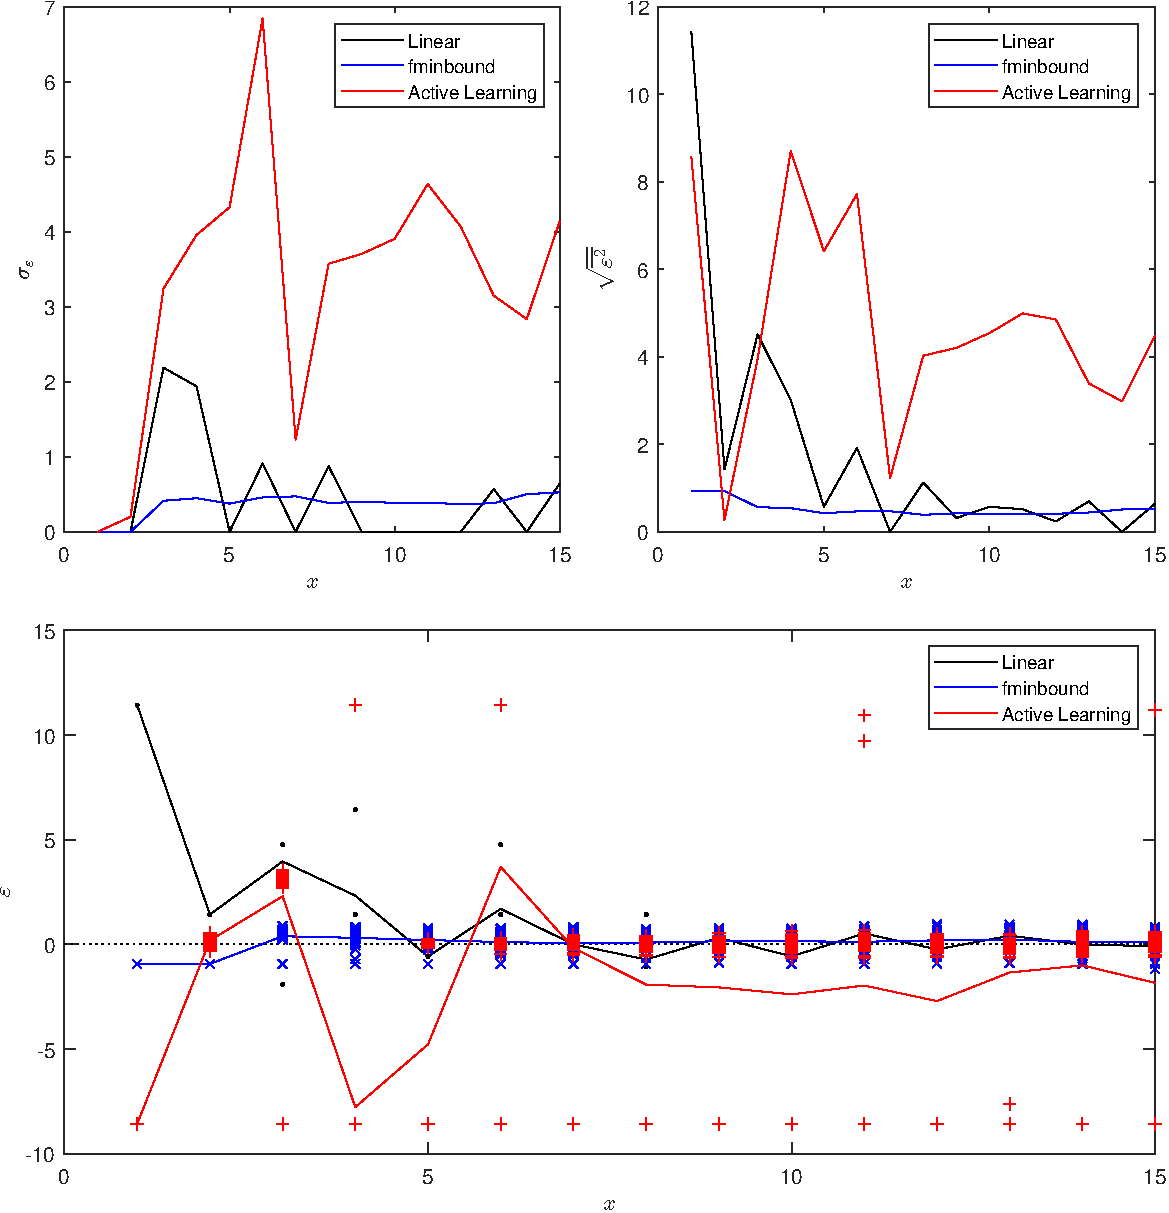
\includegraphics[width=1.0\textwidth]{comparison1.pdf}
  \caption[First Comparison]{Comparison of the three methods discussed. The top left shows the standard deviation of each method, the top right shows the absolute mean error, and the bottom shows the true error of each sample with a mean of the error to guide the eye.}
  \label{fig:firstComparison}
\end{figure}

\section{Deeper Analysis}
\subsection{Random Function}
To fully test these methods, random functions are used. For this, several basic assumptions are made:
\begin{itemize}
  \item The function is continuous.
  \item $x\in[-10, 10]$.
  \item $f(-10)=0$.
  \item $f^{\prime}(x)\sim N(0, 0.5^2)$.
  \item No additional error is attached (very noisy anyway).
\end{itemize}
A simple script for this is in Listing~\ref{lst:randomFunc}, which has been designed to allow for easy production of a curve that is differentiable to the $n^{th}$ degree.

\lstset{language=Python}
\lstset{frame=lines}
\lstset{caption={Funcion to generate a random continuous function.}}
\lstset{label={lst:randomFunc}}
\lstset{basicstyle=\footnotesize}
\begin{lstlisting}
  def randFunc():
      lims = [-10, 10]
      derivatives = 1
      x = np.linspace(*lims, 5000)
      f = np.zeros([derivatives + 1, len(x)])
      f[-1, :] = np.random.normal(0, 0.5, np.shape(x))

      for i in range(1, derivatives):
          f[i, 0] = np.random.uniform(-1, 1)

      for i in range(1, len(x)):
          for j in range(derivatives):
              f[j, i] = f[j, i - 1] + f[j + 1, i - 1] * (x[1] - x[0])

  return interp1d(x, f[0, :])

\end{lstlisting}

\subsection{Comparison on Random Functions}
As in Section~\ref{ssec:comp1}, a comparison between the three methods was carried out on samples sizes ranging from 2 to 25. These were tested on 50 different random functions, as generated by Listing~\ref{lst:randomFunc}. The problem specific algorithm surpassed the other methods in both metrics measured. Further, both active learning methods routinely surpassed fminbound. This is likely due to fminbound finding local minima and converging upon these rather than exploring the remainder of the function.

\begin{figure}[htbp!] 
  \centering    
  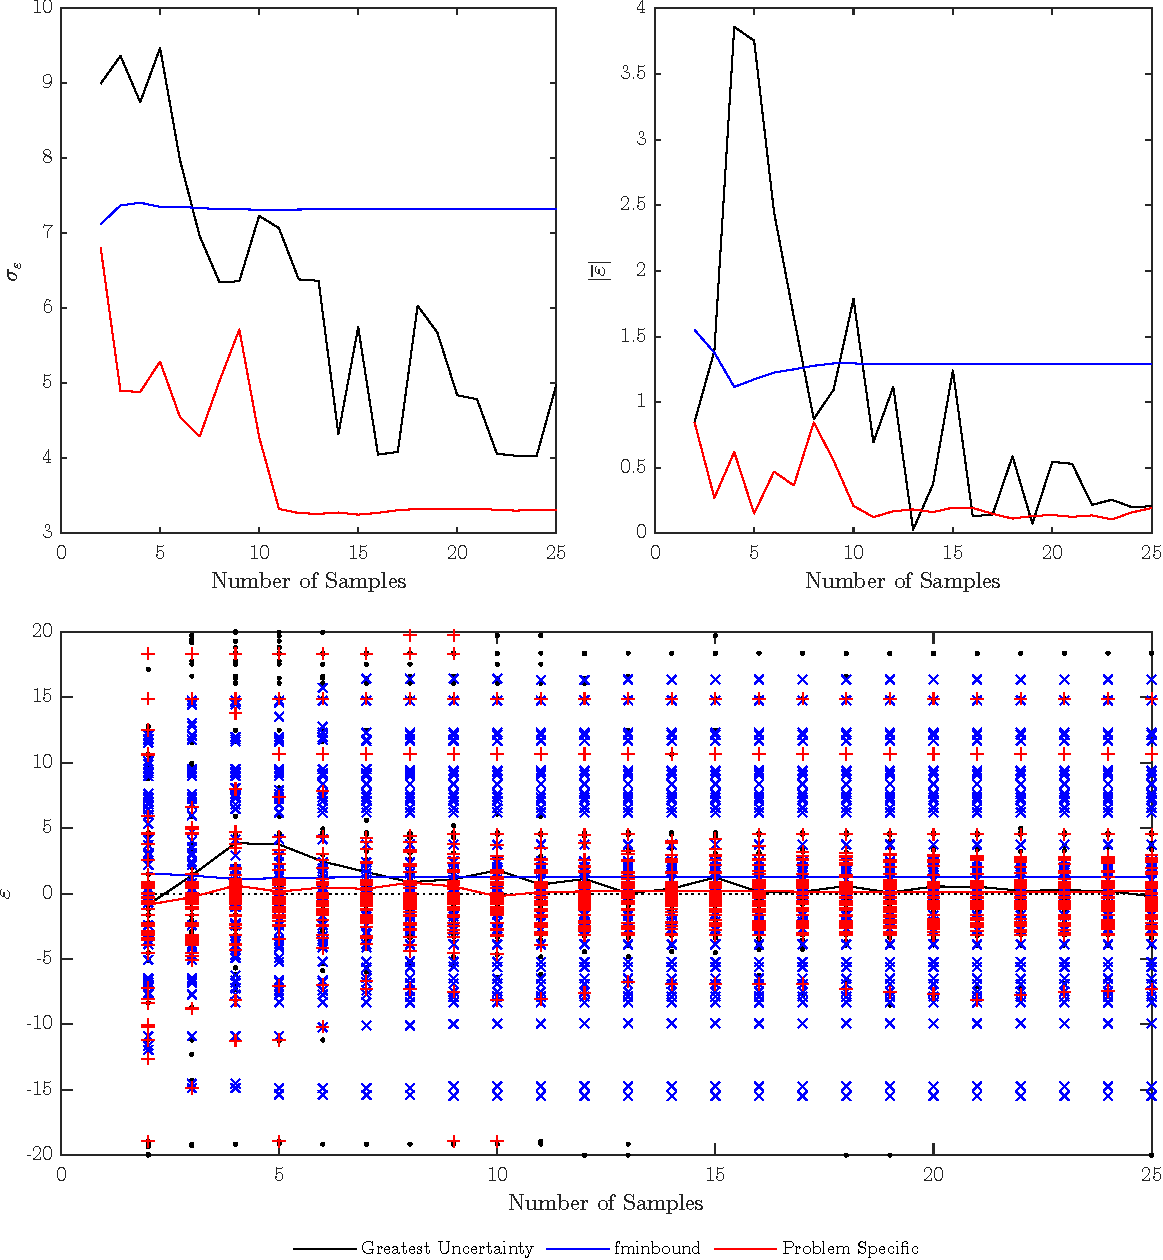
\includegraphics[width=1.0\textwidth]{comparison2.pdf}
  \caption[Rigorous Comparison]{Comparison of the three methods discussed against random functions. The top left shows the standard deviation of each method, the top right shows the absolute mean error, and the bottom shows the true error of each sample with a mean of the error to guide the eye.}
  \label{fig:betterComparison}
\end{figure}